\chapter{Method and Datasets}
\label{sec:method}
In this chapter, the specific neural network used to denoise \gls{ct} images will be introduced, some image comparison metrics will be given alongside a brief discussion of them, the used datasets will be described, and the method used to compile a given dataset into a suitable format for the neural network will be explained. 


\section{TomoGAN}
\label{sec:method:tomogan}
The denoising neural network used in this thesis is called TomoGAN \cite{liu2020tomogan}. It is a \gls{gan} where the generator is based on the U-net model (see \cref{sec:ml:types:encoderdecoder}) \cite{unet}, and the input to the \gls{gan} is not random noise but rather noisy images. There are a number of key differences in the generator from the U-net model, namely \cite{liu2020tomogan}:
\begin{itemize}
    \item There are three (instead of four) down and up sampling layers.
    \item All convolutions have zero-padding to keep image dimensions unchanged during convolutions.
    \item The generator input is a stack of $d$ adjacent slices where eight $1\times1$ convolutions are applied. 
\end{itemize}
In the down sampling part of the generator, three sets of two $3\times3$ convolutional layers with ReLU activation functions extract feature maps. Between each set of convolutional layers there is a $2\times2$ max pooling layer, for a total down sampling of $8$ leading to a feature map of size $1/8$ of the original image in either dimension (e.g. images of dimensions $1024\times1024$ will result in a feature map of dimensions $128\times128$). The number of channels in a convolutional layer changes throughout the network beginning with $8$ channels, and the feature map after the down sampling process has $128$ channels. 

The up sampling part of the generator is symmetric to the down sampling part, containing three sets of two $3\times3$ convolutional layers. The max pooling layers are replaced by bi-linear interpolation layers that instead of reducing the size of the feature map, increase it. Again, all the convolutional kernels have kernels of size $3\times3$ and use ReLU activation functions. At each of the three sets of convolutional layers, the feature maps from the corresponding set in the down sampling section are concatenated to the feature maps outputted from the previous set of convolutional layers.\footnote{These skip-connections, as they are often called, are what make this structure a U-net style network and not simply an encoder-decoder network \cite{unet}. } Finally, a $1\times1$ convolutional layer with a ReLU activation function followed by a $1\times1$ convolutional layer with a linear activation function is used to combine all the channels into a final output image. 

Because of the three $2\times2$ max pooling layers, the dimensions of the input images must all be divisible by $2^3=8$. 

A schematic of the generator of TomoGAN is provided in \cref{fig:tomoganstructure}.

\begin{figure}[htbp]
    \centering
    \includegraphics[width=0.95\textwidth]{figures/tomoganstructure.png}
    \caption[Visualization of the structure of TomoGAN]{A visualization of the structure of TomoGAN. Here, an image of size $1024\times1024$ has been used as an example. Every bar corresponds to a multi-channel feature map with the number of channels written above and the dimension of the feature map written on the bottom left. All convolutions use zero-padding. The type of activation function used with a given convolution can be seen in the legend. The copy operations transfer the feature map from a down sampling layer and concatenates it to the corresponding up sampling layer. Figure adapted from \cite{liu2020tomogan}. } 
    \label{fig:tomoganstructure}
\end{figure}

The discriminator network used to help train TomoGAN consists of six 2D $3\times3$ convolutional layers with leaky ReLU activation functions, as well as two fully connected layers. 

No changes have been made to the structure of the TomoGAN network in this thesis, however some changes have been made to the loss function used to train the network. The original TomoGAN network, as given by Liu \textit{et al.} \cite{liu2020tomogan}, was trained using a loss function comprising of an \gls{mse} loss, a feature based (VGG) loss, and an adversarial loss, given as 
\begin{equation}
    L_{\text{Total}} = \lambda_{\text{MSE}}L_{\text{MSE}} + \lambda_{\text{VGG}}L_{\text{VGG}} + \lambda_{\text{Adv}}L_{\text{Adv}}.
\end{equation}
Based on articles citing the log-cosh loss function as a good candidate for image processing \cite{7797130,chen2019log}, a log-cosh loss function (see \cref{sec:ml:training:lossfunctions}) was added as an additional term to the total loss, giving the new loss function
\begin{equation}
    L_{\text{Total}} = \lambda_{\text{MSE}}L_{\text{MSE}} + \lambda_{\text{Log-cosh}}L_{\text{Log-cosh}} + \lambda_{\text{VGG}}L_{\text{VGG}} + \lambda_{\text{Adv}}L_{\text{Adv}}.
\end{equation}
The weights for the different loss functions were mostly unchanged, with only $\lambda_\text{MSE}$ being slightly reduced to account for the fact that $L_\text{Log-cosh}$ covers a similar role (as they have similar activations). 

The TomoGAN network performs what is known as \textit{image-to-image translation}, meaning it translates one possible representation of an image into another \cite{pang2021imagetoimage,isola2018imagetoimage}.

\section{Image Comparison Metrics}
\label{sec:method:metrics}
To quantify the performance of the denoising method, some metrics must be defined. While there are some standards to doing this, not all methods perform equally well. 

\subsection{Mean Squared Error}
\label{sec:method:metrics:mse}
The most commonly used \textit{full-reference} image quality metric is the \glsfirst{mse}, as defined (as a loss function) in \cref{eq:lossmse}. While it provides some sense of similarity and is easy to calculate and physically understand, a low (i.e. good) \gls{mse} does not necessarily correspond to a high degree of visual similarity and it is therefore not a good metric to compare visual similarities in images \cite{413502,477498}. Likewise, the \gls{psnr}, which is another very commonly used metric, does not correspond to visual similarity \cite{477498}. 

\subsection{Structural Similarity Index Measure}
The \gls{ssim} is a metric to measure similarity between images \cite{ssim}. It is a full-reference image quality assessment, meaning it compares a reference image to a low-quality image.\footnote{Other types of image quality assessments are either \textit{no-reference} where there is no reference image to compare to, or \textit{reduced-reference} where there is some partial information from a reference image to compare to (e.g. a set of extracted features)\cite{ssim}. }

The \gls{ssim} takes into account three metrics of the image, namely: luminance, contrast, and structure. They are combined, giving the definition of \gls{ssim} as \cite{ssim}
\begin{equation}
    \label{eq:ssim}
    \text{SSIM}\left(x,y\right) = \frac{\left( 2\mu_x \mu_y + C_1 \right) \left( 2\sigma_{xy} + C_2 \right)}{\left( \mu_x^2 + \mu_y^2 + C_1 \right) \left( \sigma_x^2 + \sigma_y^2 + C_2 \right)},
\end{equation}
where $x$ and $y$ are the two images to compare, $\mu_{\{x,y\}}$ is the mean pixel value of an image, $\sigma_{\{x,y\}}$ is the standard deviation of the pixel values of an image, $\sigma_{xy}$ is the covariance of two images, and $C_{\{1,2\}}$ are regularization constants. It is symmetric (i.e. $\text{SSIM}\left(x,y\right) = \text{SSIM}\left(y,x\right)$), bounded (i.e. $\text{SSIM}\left(x,y\right) \leq 1$), and has a unique maximum (i.e. $\text{SSIM}\left(x,y\right) = 1$ if and only if $x = y$) \cite{ssim}. A more robust analysis of the mathematical properties of the \gls{ssim} was performed in \cite{6059504}.


\section{Datasets}
\label{sec:method:datasets}
A selection of different datasets have been used to train and test the TomoGAN network. Some of these have been collected from TomoBank \cite{TomoBank}, one is collected in-house, and one is from the ID16B beamline at the European Synchrotron Radiation Facility (ESRF). This section will give a description of each used dataset. 

The chosen datasets have been selected to represent several different \gls{ct} imaging challenges and situations. The borosilicate glass spheres dataset was chosen as an ideal beamline dataset where there is access to a high-quality dataset to properly train TomoGAN. The soda lime glass spheres dataset was chosen to examine the feasibility of using TomoGAN for dynamic \gls{ct} datasets, and to compare TomoGAN to a reconstruction based denoising technique, namely \gls{piccs}. Finally, the Pierre shale dataset was chosen because shale samples are in general hard to study with \gls{ct}, as they are composed of several minerals with similar attenuation values, making segmentation and further analysis hard. Furthermore, the Pierre shale dataset does not have a corresponding high-quality dataset to train TomoGAN, instead requiring other datasets to be used to train TomoGAN to attempt denoising. 

\subsection{Borosilicate Glass Spheres and TomoBank}
\label{sec:method:datasets:tomo00058}
TomoBank is an X-ray tomography data bank providing experimental and simulated datasets with the aim to foster collaboration among computational scientists, beamline scientists, and experimentalists \cite{TomoBank}. It provides several types of datasets imaging different samples as well as simulated phantoms. Some of these datasets have been used in this thesis.

The tomo\_00058 dataset is a dataset imaging borosilicate glass spheres encased in a polypropylene matrix \cite{datasetglassspheres}. It contains a $20\%$ concentration of glass spheres. The technical information of the dataset is given in \cref{tab:tomo00058}, and an overview of how many projections are used in different subsamplings to simulate artifacting due to undersampling is given in \cref{tab:projectionsubsampling}. The subsampling is done with evenly angular spacing. 

This dataset will be referred to as the borosilicate glass spheres dataset. An arbitrary slice of this dataset, with and without simulated undersampling artefacts, is provided in \cref{fig:tomo00058datasetexample}. 

\begin{table}[htbp]
    \centering
    \caption[Technical information of the borosilicate glass spheres dataset]{Technical information of the borosilicate glass spheres dataset. The dataset was scanned at the Advanced Photon Source (APS) at Argonne National Laboratory, USA. Further details are available from \cite{datasetglassspheres}. }
    \label{tab:tomo00058}
    \begin{tabular}{ll}
    \hline
    Beamline & APS 2-BM-A\\
    Sample rotation ranges & 180 degrees \\
    Number of projections & 1500 \\
    Energy & \SI{27.4}{\kilo \electronvolt}\\
    Exposure time & \SI{1}{\milli \second}\\
    Pixel size & \SI{0.65}{\micro \meter} \\
    Detector dimension x & 2560 \\
    Detector dimension y & 2160 \\
    \hline
    \end{tabular}
\end{table}

\begin{table}[htbp]
    \centering
    \caption[Projection subsampling overview for reconstructions of the borosilicate glass spheres dataset.]{Overview of the number of projections for different subsampling factors of the borosilicate glass spheres dataset. }
    \label{tab:projectionsubsampling}
    \begin{tabular}{ll}
    \hline
    Subsampling factor & Projections \\
    \hhline{==}
    $1$ & $1500$ \\
    $8$ & $187$ \\
    $16$ & $93$ \\
    $32$ & $46$ \\
    $48$ & $31$ \\
    \hline
    \end{tabular}
\end{table}

\begin{figure}
    \begin{subfigure}[t]{.45\textwidth}
      \centering
      \includegraphics[width=\linewidth]{figures/gt32.png}
      \caption{High-quality reconstruction (1500 projections)}
    \end{subfigure}
    \hfill
    \begin{subfigure}[t]{.45\textwidth}
      \centering
      \includegraphics[width=\linewidth]{figures/ns32.png}
      \caption{Undersampled projections (46 projections)}
    \end{subfigure}
    \caption[Borosilicate glass spheres dataset]{Different reconstructions of the borosilicate glass spheres dataset. The two images are of the same arbitrary slice from the datasets. }
    \label{fig:tomo00058datasetexample}
\end{figure}

Two datasets of shale from TomoBank were also used, namely tomo\_00001 and tomo\_00002 \cite{datasetshale}. These datasets are two shale samples collected from the North Sea and from the Upper Barnett Formation in Texas. They are both imaged at the Advanced Photon Source (APS) of Argonne National Laboratory, USA. These datasets are only used to train a network for denoising of another shale sample, namely the Pierre shale sample (see \cref{sec:method:datasets:shale}). 

All datasets used from TomoBank were reconstructed using \gls{fbp} from the TomoPy library \cite{tomopy}. 

\subsection{Soda Lime Glass Spheres}
\label{sec:method:datasets:inhouse}
An in-house captured dataset imaging a sample of soda lime glass spheres in a capillary tube containing a potassium iodide (KI) doped water solution has been used. The soda lime glass spheres have diameters ranging \SIrange{1250}{1650}{\micro \meter}, the capillary tube has an inner diameter of \SI{2.5}{\milli \meter} and an outer diameter of \SI{4.0}{\milli \meter}, and the potassium iodide doped water has a concentration of \SI{0.5}{\molar} KI. The sample was imaged twice: one slow \acrlong{hq} imaging, and one fast \acrlong{lq} imaging. The technical information of the two imagings of the in-house dataset is given in \cref{tab:inhousehq,tab:inhouselq}.

\begin{table}[htbp]
    \centering
    \caption[Technical information of the IHHQ soda lime glass spheres dataset]{Technical information of the \acrlong{hq} imaging of the in-house dataset. }
    \label{tab:inhousehq}
    \begin{tabular}{ll}
    \hline
    Instrument & Nikon XT H 225 ST \\
    Number of projections & 1570 \\
    Voltage & \SI{170}{\kilo \volt}\\
    Current & \SI{45}{\micro \ampere}\\
    Gain & \SI{17}{\deci \bel}\\
    Exposure time & \SI{1000}{\milli \second}\\
    Pixel size & \SI{7.06}{\micro \meter} \\
    \hline
    \end{tabular}
\end{table}

\begin{table}[htbp]
    \centering
    \caption[Technical information of the IHLQ soda lime glass spheres dataset]{Technical information of the fast scan of the in-house dataset. }
    \label{tab:inhouselq}
    \begin{tabular}{ll}
    \hline
    Instrument & Nikon XT H 225 ST \\
    Number of projections & 150 \\
    Voltage & \SI{170}{\kilo \volt}\\
    Current & \SI{65}{\micro \ampere}\\
    Gain & \SI{24}{\deci \bel}\\
    Exposure time & \SI{134}{\milli \second}\\
    Pixel size & \SI{7.06}{\micro \meter} \\
    \hline
    \end{tabular}
\end{table}

For the sake of simplicity, the two datasets will be referred to as the \gls{ihhq} and the \gls{ihlq} datasets. 

Because the used \gls{ct} instrument has a conical beam, the \gls{fdk} reconstruction algorithm was used to reconstruct these datasets. A \gls{piccs} reconstruction of the \gls{ihlq} dataset is also included as an alternative denoising method for comparison. 

A figure showing an arbitrary slice from the \gls{ihhq}, \gls{ihlq}, and \gls{ihlq} \gls{piccs} datasets is provided in \cref{fig:kimrobertdatasets}.

\begin{figure}
    \begin{subfigure}[t]{.31\textwidth}
      \centering
      \includegraphics[width=\linewidth]{figures/kimrobertgt.png}
      \caption{\gls{ihhq}. }
    \end{subfigure}
    \hfill
    \begin{subfigure}[t]{.31\textwidth}
      \centering
      \includegraphics[width=\linewidth]{figures/kimrobertFDK.png}
      \caption{\gls{ihlq} \gls{fdk}.}
    \end{subfigure}
    \hfill  
    \begin{subfigure}[t]{.31\textwidth}
      \centering
      \includegraphics[width=\linewidth]{figures/kimrobertPICCS.png}
      \caption{\gls{ihlq} \gls{piccs}. }
    \end{subfigure}
    \caption[IHHQ and IHLQ soda lime glass spheres dataset]{Different reconstructions of the \gls{ihhq} and \gls{ihlq} soda lime glass spheres datasets. The three images are of the same arbitrary slice from the datasets. }
    \label{fig:kimrobertdatasets}
\end{figure}

\subsection{Pierre Shale}
\label{sec:method:datasets:shale}
\todo[inline]{Get the technical information of this dataset}
This sample is a piece of Pierre shale, measured with phase-contrast \gls{ct} at the beamline ID16 at the European Synchrotron Radiation Facility (ESRF). 

\begin{table}[htbp]
    \centering
    \caption[Technical information of the Pierre shale dataset]{Technical information of the Pierre shale dataset. The dataset was scanned at the ID16B beamline at the European Synchrotron Radiation Facility (ESRF). }
    \label{tab:pierreshale}
    \begin{tabular}{ll}
    \hline
    Beamline & ESRF ID16 \\
    Sample rotation ranges &  \\
    Number of projections &  \\
    Energy & \\
    Exposure time & \\
    Pixel size & \\
    Detector dimension x &  \\
    Detector dimension y &  \\
    \hline
    \end{tabular}
\end{table}

\begin{figure}[htbp]
    \centering
    \includegraphics[width=.45\textwidth]{figures/shale/shale_ns/0.png}
    \caption[Pierre shale dataset]{View of the Pierre shale dataset. No high-quality reconstruction is available. }
    \label{fig:shaledataset}
  \end{figure}


\section{Compiling a Dataset for Training}
\label{sec:method:compilingdataset}
In this section, an explanation of how to compile a set of images into a suitable dataset for training the TomoGAN network, or to denoise with an already trained network, will be presented. 

The process of preparing a dataset for either training or inference (i.e. denoising using an already trained network) consists of a few steps. A flowchart visualizing this process is provided in \cref{fig:compilingdatasetflowchart}. The detailed steps are as follows:

\begin{enumerate}
    \item Begin with a full stack of reconstructed images. If the dataset is meant to be used to train the network, both a set of \gls{hq} reconstructions as well as a corresponding set (of the same dataset) of \gls{lq} reconstructions are needed. They must be sorted the same way so that image 0 of the \gls{hq} dataset corresponds to image 0 of the \gls{lq} dataset. If it is a dataset that is to be denoised, only the \gls{lq} dataset is needed. 
    \item The images must then be cropped to remove unnecessary empty space and to help the network pick up on the important parts of the image. For a dataset that has not been properly cropped, the network may struggle to converge to a good solution, yielding poor results. This cropping step is done by visually inspecting the dataset and cropping an appropriate part of the images. If the dimensions of the images are very large, it may be too large to properly fit in memory during training or denoising. The images must then be resized to an appropriate smaller size. The dimensions must also be divisible by $8$ (see \cref{sec:method:tomogan}).
    \item Once the images are cropped, they must be converted to the datatype uint8, as that is best suited for use in the network.\footnote{Using uint8 instead of e.g. float32 reduces the memory footprint drastically, and the hardware used to perform the calculations needed to train a neural network is often optimized for this type of calculations using uint8. } This process consists of several steps. For each image in the dataset do the following:
    \begin{enumerate}
        \item First, find the minimum and maximum pixel values of an image. This can be the absolute minimum and maximum, but ideally it should be a lower and upper percentile of the pixel values to avoid single extreme pixel values causing a loss of dynamic range in the image, as the pixel values will be limited to 256 distinct values. 
        \item Once the minimum and maximum values are determined, the image pixel values should be clipped to the previously determined minimum and maximum values. This is necessary when the minimum and maximum values are percentiles to ensure all pixel values are within the new value range set by the percentiles.
        \item After clipping the pixel values, all pixel values can be scaled linearly between 0 and 255 according to the formula 
        \begin{equation}
            \label{eq:scaleimages}
            \hat{x} = 255 \cdot \frac{x - I_{min}}{I_{max} - I_{min}},
        \end{equation}
        where $\hat{x}$ is the updated scaled pixel value, $x$ is the old pixel value, and $I$ is the whole image.
    \end{enumerate}
    \item Once all images are scaled and converted to uint8, they can be filled into an HDF5-file containing one dataset for the \gls{hq} images, and if the dataset is to be used to train the network, one dataset for the \gls{lq} images. The dimensions of the datasets should be $(N,H,W)$, where $N$ is the number of images, and $(H,W)$ are the dimensions of the images. 
    \item When the dataset is to be used to train the network, both the \gls{hq} and the \gls{lq} datasets must be split into two datasets: one for training, and one for testing. About $15\%$ of the total dataset should be set aside for testing. If the depth parameter of TomoGAN is to be used, both the training and test datasets need to be sorted (i.e. adjacent slices are adjacent in the dataset). 
\end{enumerate}


\begin{figure}[htbp]  
    \centering
    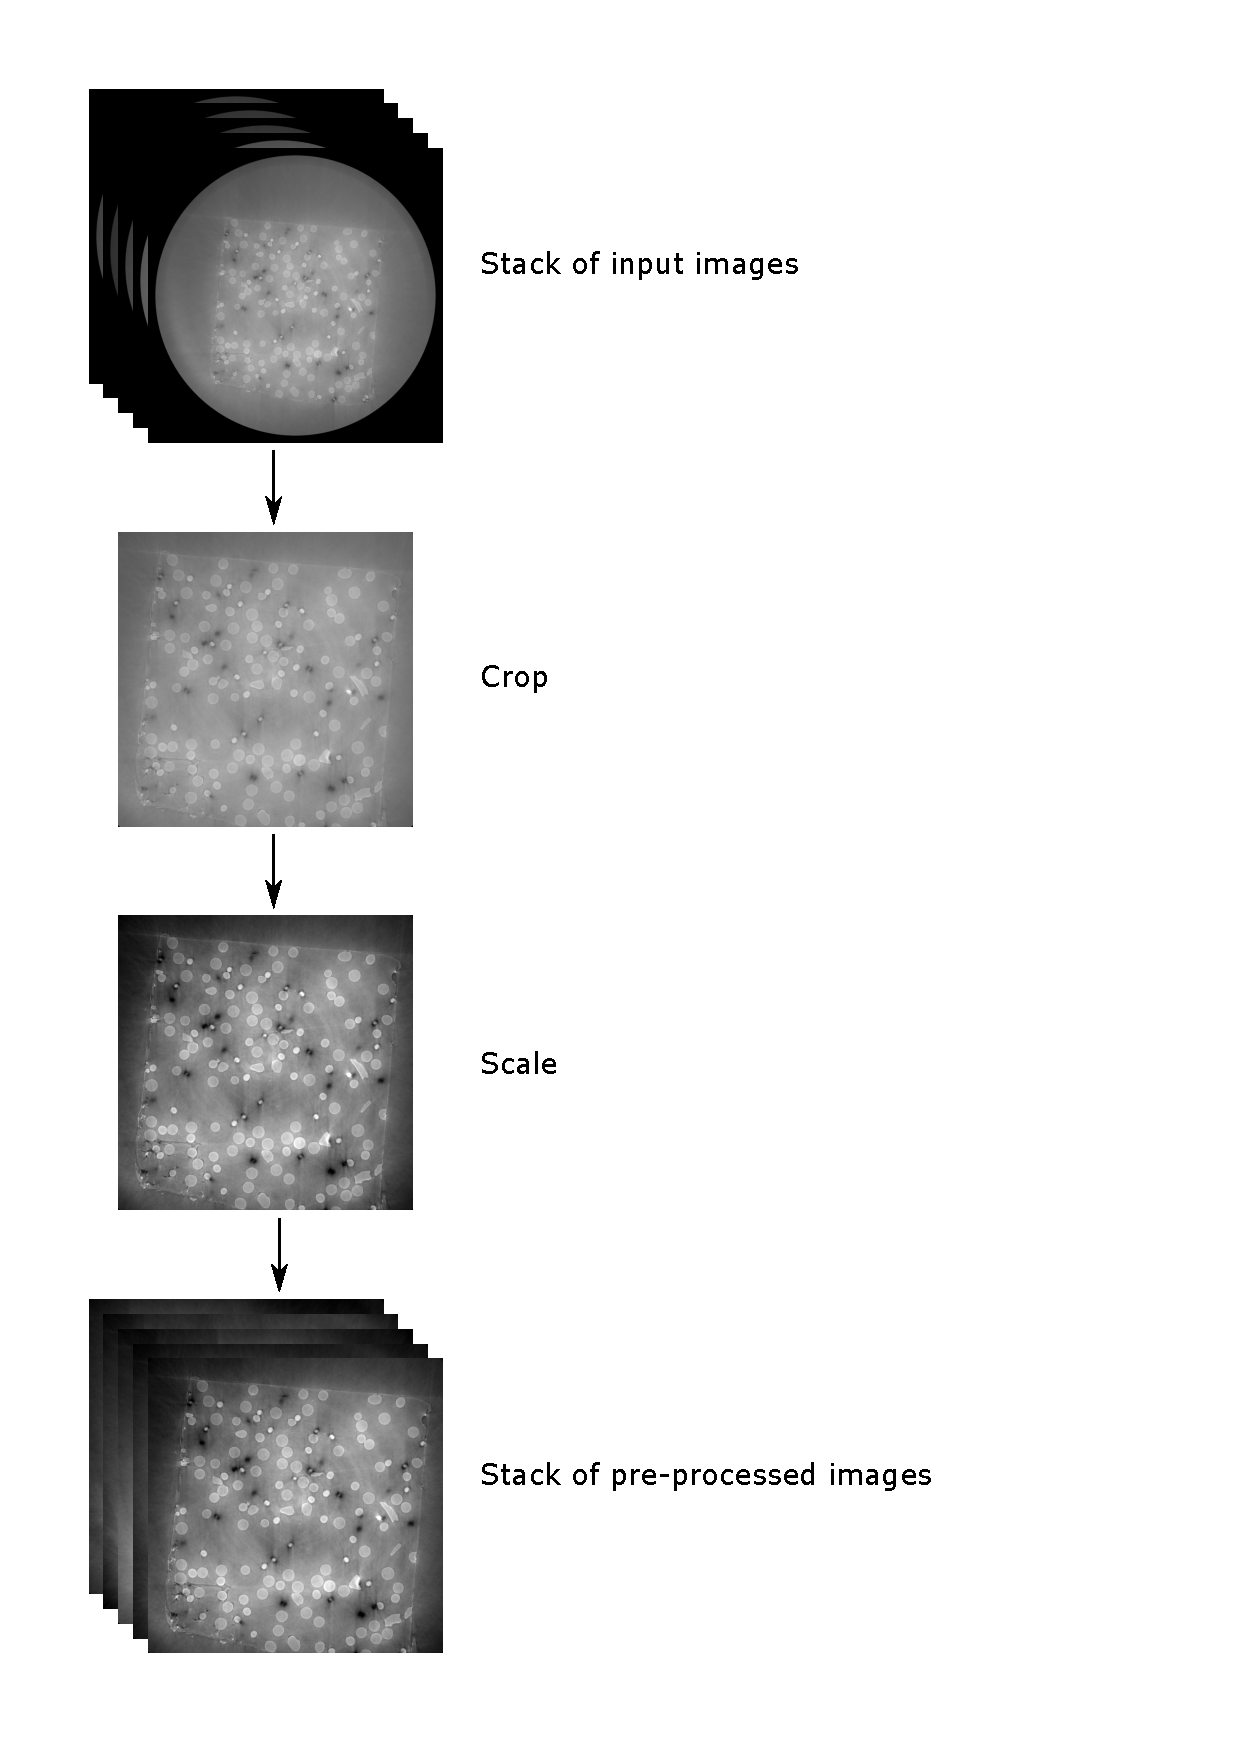
\includegraphics[width=.95\textwidth]{figures/compilingdatasetflowchart.pdf}
    \caption[Dataset creation flowchart for TomoGAN]{Flowchart showing the process of compiling a dataset for training the TomoGAN denoising network. See \cref{sec:method:compilingdataset} for a thorough explanation. }
    \label{fig:compilingdatasetflowchart}
\end{figure}
